\makeatletter
\renewcommand{\@noticestring}{}  % removes the conference notice
\makeatother

\documentclass{article}


% if you need to pass options to natbib, use, e.g.:
%     \PassOptionsToPackage{numbers, compress}{natbib}
% before loading neurips_2023


% ready for submission
\usepackage[final]{main}


% to compile a preprint version, e.g., for submission to arXiv, add add the
% [preprint] option:
%\usepackage[preprint]{neurips_2023}


% to compile a camera-ready version, add the [final] option, e.g.:
%     \usepackage[final]{neurips_2023}


% to avoid loading the natbib package, add option nonatbib:
%    \usepackage[nonatbib]{neurips_2023}


\usepackage[utf8]{inputenc} % allow utf-8 input
\usepackage[T1]{fontenc}    % use 8-bit T1 fonts
\usepackage{hyperref}       % hyperlinks
\usepackage{url}            % simple URL typesetting
\usepackage{booktabs}       % professional-quality tables
\usepackage{amsfonts}       % blackboard math symbols
\usepackage{graphicx}       % for including graphics
\usepackage{nicefrac}       % compact symbols for 1/2, etc.
\usepackage{microtype}      % microtypography
\usepackage{xcolor}         % colors


\title{AI Live Analytics Generator}


% The \author macro works with any number of authors. There are two commands
% used to separate the names and addresses of multiple authors: \And and \AND.
%
% Using \And between authors leaves it to LaTeX to determine where to break the
% lines. Using \AND forces a line break at that point. So, if LaTeX puts 3 of 4
% authors names on the first line, and the last on the second line, try using
% \AND instead of \And before the third author name.


\author{
  Pranav Turlapati \quad
  Vamsi Palukuri \quad
  Sujay Patel \quad
  Prateek Mishra \quad
  Ishaan Balakrishnan \\
  University of North Carolina at Chapel Hill \\
  pran@unc.edu, vamsip@unc.edu, sujayp@unc.edu, prateekm@unc.edu, ishaanb@unc.edu
}



\begin{document}


\maketitle


\begin{abstract}
  While statistics and analytics have been extensively applied in sports analyses, leveraging real-time speech and commentary data to generate meaningful visual analytics in Sports games remains underexplored. In this paper, we propose a novel approach that integrates audio event recognition, large language models (LLMs), and statistical visualization techniques to enhance the understanding of basketball events in real time. Our method captures live commentary, segments speech based on semantic transitions between game events, and utilizes an LLM to determine whether specific segments warrant visualization. By converting spoken descriptions into structured variables—such as player identities, relevant statistics, and team information—we dynamically generate insightful visualizations. To ensure the reliability of our outputs, we further develop a classification model trained to predict potential inaccuracies in the decision-making process, significantly reducing erroneous visualizations. Experimental results demonstrate that our proposed method outperforms conventional real-time analytics approaches, providing more accurate and contextually relevant visualizations. Our framework offers a practical solution for augmenting live sports broadcasts with analytically meaningful, real-time graphical insights derived from natural language commentary.

\end{abstract}


\section{Introduction}

\paragraph{Data}

Our study utilizes highlight segments from NBA basketball games sourced from YouTube
videos of the most recent season. We randomly selected 20 different NBA games, each
containing approximately 40 distinct speech segments, or plays, on average. Each data
point comprises one to two sentences of commentary describing a specific play. To efficiently
preprocess this data, we employed a large language model (LLM) to segment YouTube
transcripts into meaningful commentary units, facilitating easy scalability for larger datasets.
1
These segments provide rich descriptive information from announcers, capturing details of
player actions, team interactions, and key game events, serving as the foundational data for
our real-time analytics and visualization framework.

We utilized real-time basketball data from the NBA 2024-2025 season, specifically sourced
from comprehensive box scores available through the NBA API. The dataset includes de-
tailed box scores for each NBA game played during the season, comprising essential player
performance statistics. Each entry contains data points such as GAME ID (unique iden-
tifier for each game), TEAM ID (unique identifier for teams), TEAM ABBREVIATION,
TEAM CITY, PLAYER ID (unique identifier for each player), PLAYER NAME, and PLAYER NICKNAM
The dataset also includes specific gameplay metrics: minutes played (MIN), field goals
made (FGM) and attempted (FGA), field goal percentage (FG PCT), three-point shots
made (FG3M) and attempted (FG3A), three-point percentage (FG3 PCT), free throws
made (FTM) and attempted (FTA), free throw percentage (FT PCT), offensive rebounds
(OREB), defensive rebounds (DREB), total rebounds (REB), assists (AST), steals (STL),
blocks (BLK), turnovers (TO), personal fouls (PF), points scored (PTS), and plus-minus
(PLUS MINUS).
This comprehensive statistical dataset provides detailed insights into player and team
performance throughout the NBA season, serving as the foundational data source for gen-
erating meaningful real-time visual analytics.

\paragraph{Motivation and Goals}

The rising popularity of sports broadcasts has highlighted the increasing need for contextual and analytically-driven commentary to enhance viewer engagement and comprehension. Current sports commentary often lacks detailed statistical context, leaving fans, analysts, and sports bettors seeking deeper insights into game dynamics and player performances. For instance, when commentators mention a player "taking a step up," specific numerical support such as their points per game (PPG) would significantly enrich viewers' understanding of such claims.

Furthermore, integrating comprehensive analytics and real-time visualizations can reduce inherent biases in commentary, especially those influenced by announcers' affiliations with certain teams. Objective, data-driven insights can provide a balanced perspective, offering viewers a clearer and more accurate picture of the game's progression.

Additionally, sports bettors and dedicated fans frequently seek detailed statistics and predictive analyses beyond basic play-by-play commentary. Queries like how often the Los Angeles Lakers win when LeBron James scores ten or more points in the first quarter demonstrate a clear demand for sophisticated statistical context and predictive insights.

To address these gaps, our project leverages audio recognition, large language models (LLMs), and statistical visualization methods to dynamically enrich basketball broadcasts with real-time analytics. Our approach aims to enhance viewer experience by providing meaningful statistical insights, reducing commentator bias, and satisfying the analytical curiosity of sports enthusiasts and bettors.

We selected NBA basketball specifically due to the high frequency of plays per game, offering abundant opportunities for real-time analytics. Although other sports like football also have numerous plays, the clear temporal separation between plays in football already simplifies real-time analytics, resulting in extensive existing solutions. Additionally, the NBA provides a comprehensive and publicly available database of player statistics, further supporting robust analytics and visualization.

\section{Methods}

\paragraph{Audio Segmentation with Whisper}
Our methodology begins with audio segmentation using OpenAI's Whisper model, an advanced automatic speech recognition system designed to transcribe and segment speech accurately. Whisper processes audio streams, efficiently identifying meaningful speech segments within short intervals (approximately 5 seconds). We selected Whisper for its robustness and reliability in handling varied speech patterns, ambient noise, and overlapping conversations common in sports commentary.

\paragraph{Text-to-Variable Conversion via GPT-4 Mini}
Each segmented audio clip from Whisper is then fed into GPT-4 mini, a powerful generative AI model. GPT-4 mini interprets the textual commentary, extracting structured variables essential for visualization decisions: whether a graph should be created, the type of graph (team-focused or player-focused), the home and away teams, the player's name, and the specific statistic mentioned. We chose GPT-4 mini due to its high accuracy and capability to contextualize complex, unstructured sports commentary, transforming it into actionable data.

\paragraph{Visualization Generation with Matplotlib}
The extracted variables from GPT-4 mini guide our custom-developed Python scripts utilizing Matplotlib for visualization. The scripts dynamically generate clear and informative graphs tailored to each commentary segment, providing viewers with immediate and relevant statistical insights.

\paragraph{Error Filtering via Classification Model}
To enhance accuracy and minimize erroneous visualizations, we developed a classification model based on BERT (Bidirectional Encoder Representations from Transformers). This model was trained on manually labeled commentary data, identifying instances where generated graphs were incorrect or unnecessary. By analyzing the original textual input used by GPT-4 mini, the BERT classifier effectively predicts potential visualization errors, allowing us to preemptively filter out unreliable graph generations. We chose BERT for its exceptional performance in text classification tasks, particularly for contextual and nuanced language common in sports commentary. Additionally, we prioritize omitting a potentially useful graph (false negative) rather than displaying a misleading visualization (false positive), ensuring the overall trustworthiness and accuracy of our analytics-driven visualizations.

\section{Results}

Figure 1 shows  an example of a result that would come to the screen. The commentator would say something along the lines of “OH-MY Lebron James with a HUGE block to seal the game”. Consequently, a visual of LeBron James’ blocks versus the league and opponent numbers would appear on the screen after the AI recognizes that a comment on a player’s statistics has been announced.

In Figure 2 shows an example if during game, the commentary "Alvarado fires away and buries the three" was made, the resulting structure would be returned and fed into our algorithm:

\begin{figure}
    \centering
    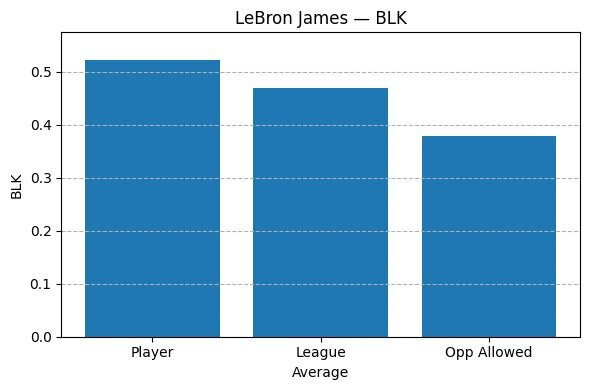
\includegraphics[width=0.5\linewidth]{LebronJames.jpg}
    \caption{Data visualization provided after commentator states that Lebron made a block.}
    \label{fig:enter-label}
\end{figure}

\begin{figure}
    \centering
    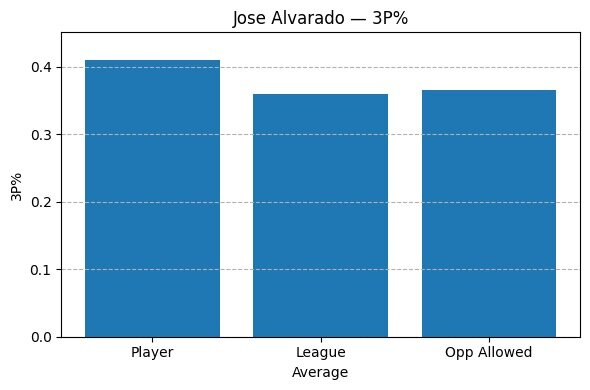
\includegraphics[width=0.5\linewidth]{JoseAlvarado.jpg}
    \caption{Data visualization provided when commentator in New Orleans Pelicans, Brooklyn Nets game said "Alvarado fires away and buries the three."}
    \label{fig:enter-label}
\end{figure}
\begin{quote}
\verb|algo({"team":"BKN","opponent":"NOP","graph":true,|
\verb|"player_graph":true,"players":["Jose Alvarado"],|
\verb|"player_stat":"3P%","team_stat":null}, player_df, team_df)|
\end{quote}

This is relevant to our problem since the viewer would likely wonder how the player has performed in such situations before. When Alvarado hits a 3-pointer, they likely search on Google or another engine for his 3-point percentage along with some more additional searches on other players to get a sense of how good he is playing in comparison to others in the league. Delivering these quick results in real-time would be beneficial for the viewer and their contextual knowledge of the situation.


\section{Conclusion}

Our approach successfully integrated audio segmentation, large language models, statistical visualization, and error filtering to enhance real-time analytics in NBA basketball broadcasts. Whisper effectively segmented commentary audio into actionable speech segments, while GPT-4 mini accurately translated these segments into structured variables essential for generating meaningful visual analytics. Matplotlib efficiently transformed these variables into insightful and contextually relevant visualizations, significantly enriching the viewer experience.

However, the current implementation exhibits a noticeable delay—on the order of a few seconds—primarily due to the speed of audio segmentation and speech-to-text conversion by Whisper, presenting a critical area for improvement to ensure seamless real-time analytics during live broadcasts.

The incorporation of a BERT-based classification model proved especially valuable, effectively identifying and filtering potential inaccuracies in visualization decisions. The model had a loss of 0.27 whereas initially, .23 of the data incorrectly produced a graph. Although the loss is similar to the initial error, it is important to note that initially, the error was that we were getting graphs when there should be no output for a graph, and now the loss from the model comes mostly from predicting good text (not likely to produce a wrong graph) as likely to produce a wrong graph. This is in line with our initial goal, as we would rather suppress a good graph than generate a faulty one.

Our findings emphasize the practicality and effectiveness of leveraging advanced speech recognition, generative AI, and classification models for real-time sports analytics. While deep learning models demonstrated exceptional performance in contextual understanding and visualization generation, the combination with classical ML techniques like BERT provided an optimal balance between accuracy and computational efficiency.

\paragraph{Next Steps}
Future enhancements for our project include exploring deeper neural network architectures and additional fine-tuning strategies to further reduce errors and computational overhead, thereby optimizing real-time analytics for broader applications. Introducing more advanced, context-specific statistics tailored explicitly to particular gameplay scenarios would significantly enhance the depth and relevance of the visualizations provided.

Additionally, we plan to generalize our framework to accommodate other sports, adapting our audio recognition, data extraction, and visualization methodologies to a variety of athletic contexts. This generalization would allow our approach to benefit a broader range of viewers and sports enthusiasts.

To further tailor our approach, we aim to develop specialized visualization versions catering separately to sports bettors, who require detailed predictive analytics, and casual viewers, who seek simpler, more intuitive insights. Lastly, optimizing the system for reduced latency between speech recognition and graph output will enhance the real-time experience, making our analytics more seamless and immediately actionable during live broadcasts.





%%%%%%%%%%%%%%%%%%%%%%%%%%%%%%%%%%%%%%%%%%%%%%%%%%%%%%%%%%%%

\begin{thebibliography}{9}

\bibitem{palmieri2024nba}
Eduardo Palmieri. \emph{NBA Player Stats Season 24/25}. 2024.  
\url{https://www.kaggle.com/datasets/eduardopalmieri/nba-player-stats-season-2425}. Accessed: 2025-04-30.

\bibitem{albi2024boscoscore}
Albi. \emph{NBA Boscoscore 2024-25}. 2024.  
\url{https://www.kaggle.com/datasets/albi9702/nba-boscoscore-2024-25}. Accessed: 2025-04-30.

\end{thebibliography}

\end{document}
